\documentclass[a4paper,11pt]{jsarticle}
\usepackage{amsmath, amsfonts}
\usepackage{bm}
\usepackage[dvipdfmx]{graphicx}
\usepackage{here}
\newcommand{\ywx}{y_i{\bm w}^\top{\bm x}_i}
\renewcommand{\exp}[1]{\text{exp}\left({#1}\right)}
\begin{document}
  \title{先端データ解析論 第11回小レポート}
  \author{情報理工学系研究科電子情報学専攻M1 堀 紡希 48216444}
  \date{\today}
  \maketitle
  \section*{宿題1}
  図を以下に示す.
  optimizerとしてAdamを用いたためか, loss, accuracyともに同じepochでも授業スライドで示された図よりも性能が良くなっている事がわかる.
  ソースコードを別のipynbファイルでも提出する.
  \begin{figure}[H]
    \centering
    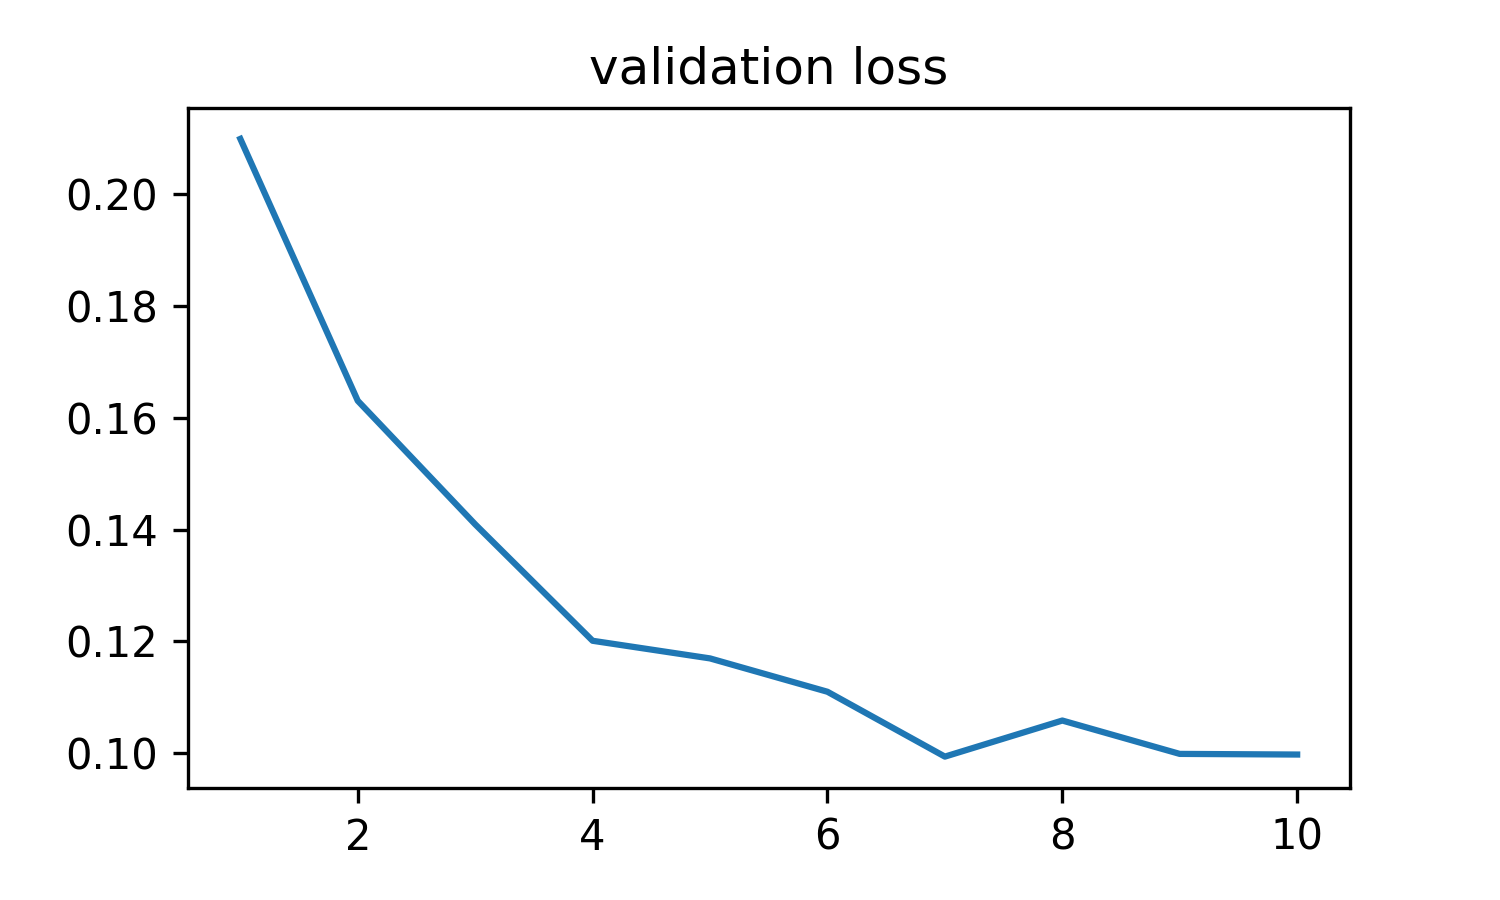
\includegraphics{loss.png}
  \end{figure}

  \begin{figure}[H]
    \centering
    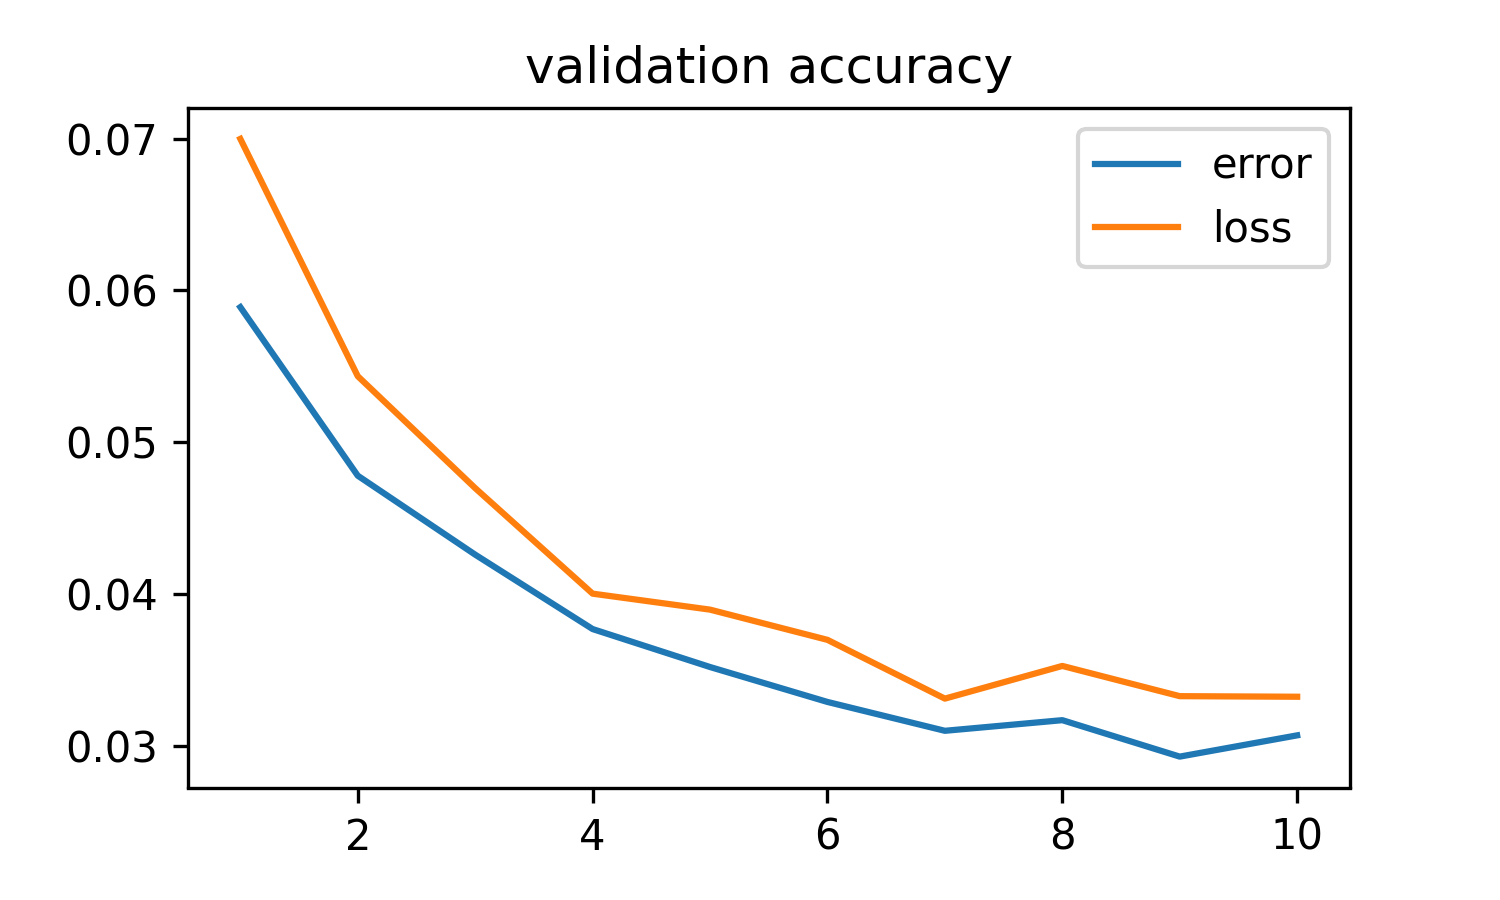
\includegraphics{accuracy.png}
  \end{figure}



  \section*{宿題2}
  多クラス分類問題において, 
  \begin{align*}
    \delta _j ^{(L)} &= \frac{\partial}{\partial u_j} \left( -\sum_{k=1}^K y_{k} \log{f_k({\bm x}; {\bm w})}\right)\\
    &= -y_j \frac{\partial}{\partial u_j}\log{f_j({\bm x}; {\bm w})} - \sum _{k \neq j} y_k \frac{\partial}{\partial u_k} \log{f_k({\bm x}; {\bm \theta})}\\
    &= -y_j \frac{\frac{\partial}{\partial u_j}f_j({\bm x}; {\bm w})}{f_j({\bm x}; {\bm w})} - \sum _{k\neq j} y_k \frac{\frac{\partial}{\partial u_j}f_k({\bm x}; {\bm w})}{f_k({\bm x}; {\bm w})}
  \end{align*}

  ここで, 
  \begin{align*}
    \frac{\partial}{\partial u_j} f_j({\bm x}; {\bm w}) &= \frac{\partial}{\partial u_j} \frac{\exp{u_j}}{\sum _k \exp{u_k}}\\
    &= \frac{\exp{u_j} \sum _{k\neq j} \exp{u_k} }{\left(\sum _k \exp{u_k}\right)^2}
  \end{align*}
  を用いると, 
  \begin{align*}
    -y_j \frac{\frac{\partial}{\partial u_j}f_j({\bm x}; {\bm w})}{f_j({\bm x}; {\bm w})} &= -y_j \frac{\exp{u_j}\sum _{k\neq j} \exp{u_k}}{\left(\sum _k \exp{u_k}\right)^2} \frac{\sum _k \exp{u_k}}{\exp{u_j}}\\
    &= -y_j \frac{\sum _{k\neq j} \exp{u_k}}{\sum _k \exp{u_k}}\\
    &= -y_j \left(1 - \frac{\exp{u_j}}{\sum _k \exp{u_k}}\right)\\
    &= -y_j (1-f_j)\\
  \end{align*}

  また$k \neq j$に対して, 
  \begin{align*}
    \frac{\partial}{\partial u_j} f_k({\bm x}; {\bm w}) &= \frac{\partial}{\partial u_j} \frac{\exp{u_k}}{\sum _l \exp{u_l}}\\
    &= -\frac{\exp{u_j} \exp{u_k} }{\left(\sum _l \exp{u_l}\right)^2}
  \end{align*}
  を用いると, 
  \begin{align*}
    - \sum _{k\neq j} y_k \frac{\frac{\partial}{\partial u_j}f_k({\bm x}; {\bm w})}{f_k({\bm x}; {\bm w})} &= \sum_{k\neq j} y_k \frac{\exp{u_j}}{\sum _l \exp{u_l}}\\
    &= \sum _{k \neq j} y_k f_j
  \end{align*}

  以上から, 
  \begin{align*}
    \delta _j ^{(L)} &= -y_j(1-f_j) + \sum _{k \neq j}y_k f_j \\
    &= \sum _{k} y_k f_j - y_j\\
    &= f_j\sum _k y_k - y_j\\
    &= f_j - y_k
  \end{align*}

\end{document}